\chapter{Die Quantitätstheorie}

Die Inflationstheorie der Monetaristen versucht die Inflation damit zu erklären, dass einem Wachstum der Güterproduktion ein zu hohes Geldmengenwachstum gegen-übersteht. Im Umkehrschluss bedeutet das, es kann durch die Steuerung der Geldmenge durch staatliche Autoritäten erreicht werden, dass Inflation oder Deflation bewusst hervorgerufen, somit gesteuert werden kann. Viele Komponenten dieser Theorie stützen sich auf die Quantitätstheorie. Im folgenden soll nun im Detail erklärt werden, wie sich die Quantitätstheorie und die damit verbundenen Quantitätsgleichungen zusammensetzen und was deren Ursachen sind. Dies stellt eine wichtige Grundlage dar, da sich so die angebotsorientierte Inflationstheorie von selbst erkennen lässt \autocite{brunner1970}.

\section{Geschichte der Quantitätstheorie}
Bereits im 16. Jahrhundert war die Idee der Quantitätstheorie vorhanden. Es wurde argumentiert, dass der Zufluss an Gold und Silber, durch neue Handelsrouten mit Asien, die Preise in Europa beeinflusste. Im Mittelalter wurde also bereits postuliert, dass die Menge der Zahlungsmittel einen Einfluss auf die Preisbildung hat \autocite{Woll1977}.

Diese Gedanken wurden dann, Anfang des 19. Jahrhunderts, wissenschaftlich bearbeitet und Ökonomen begannen, eine allgemeine Theorie zur Verhaltensbestimmung des Preises auf Basis der zur Verfügung stehenden Zahlungsmittel aufzustellen.\\
Im Jahr 1911 formulierte der Ökonom \textbf{Irving Fisher} in seiner Arbeit \enquote{The Purchasing Power of Money} die erste Version dessen, was allgemein als Quantitätstheorie bekannt ist. Der wohl bekannteste Vertreter der Neo-Quantitätstheorie ist der amerikanische Ökonom \textbf{Milton Friedman}. Die Anhänger dieser Theorie sind auch als \textbf{Monetaristen} bekannt \autocite[Kapitel~3,S.~10-12]{historyQunatitaetstheorie}.

Mit \textbf{John Maynard Keynes} findet die Quantitätstheorie einen ihrer schärfsten Kritiker, welcher behauptet, dass die Möglichkeit der Einflussnahme einer Zentralbank auf die Realwirtschaft durch Steuerung der Geldmenge nicht möglich sei. Seine nachfrageorientierte Inflationstheorie findet heute noch in Form des Keynesianismus eine große Popularität.

\section{Allgemeine Quantitätsgleichungen}

Die Quantitätstheorie vertritt den Ansatz, dass durch Steuerung der Geldmenge die Realwirtschaft beeinflusst werden kann. Genauer wird behauptet, dass sich der Preis verändert. \\
Mithilfe der Inflation, einer Erhöhung der Geldmenge, soll ein höherer Preis erreicht werden. Durch Deflation, einer Verkleinerung der Geldmenge, soll ein niedrigerer Preis erzielt werden \autocite[110]{clement1998grundlagen}. Diese Idee führt so folgenden Gleichungen:
\subsection{Transaktionsversion der Quantitätsgleichung}
\begin{equation}
    \tag{Transaktionsversion}
    M \cdot V = T \cdot P
\end{equation}\label{Transaktionsversion}

Diese Quantitätsgleichung beschreibt eine Identität zwischen dem Produkt der Geldmenge $M$ und der Geldumlaufgeschwindigkeit $V$, sowie dem Produkt der Anzahl aller Transaktionen $T$ und dem durchschnittlichen Preis $P$ dieser Transaktionen. Um die Identität etwas deutlicher zu machen, können die beiden Seiten der Gleichung folgendermaßen interpretiert werden:

\subsubsection*{Das Produkt $M \cdot V$:}
Die Geldmenge multipliziert mit der Geldumlaufgeschwindigkeit stellt nichts anderes dar, als die \enquote{Summe aller Zahlungen} in einer Realwirtschaft.

\subsubsection*{Das Produkt $T \cdot P$:}
Hierbei handelt es sich um die \enquote{Summe der Werte aller Käufe}.

\subsubsection*{Interpretation der Gleichung}
Betrachtet man die beiden Interpretationen der Identität \vref{Transaktionsversion} stellt man fest, dass die Aussage die \enquote{Summe aller Zahlung ist gleich der Summe der Werte aller Käufe} im Rahmen einer volkswirtschaftlichen Betrachtung ohne Ausnahme bejaht werden kann. Es handelt sich bei der Identität also um eine \textbf{Tautologie}.

Um nun diese Feststellung in der realwirtschaftlichen Betrachtung nutzen zu können, müssen die einzelnen Komponenten der Formel eine Bedeutung erhalten. Um z.B. die Geldmenge $M$ zu bestimmen, können bereits bekannte Größen für Geldmenge, $M_0$, $M_1$,$M_2$ oder $M_3$, herangezogen werden. Es spielt vorerst keine Rolle, welche Geldmenge betrachtet wird, sofern die Wahl der anderen Komponenten der Gleichung mit Beachtung dieser Entscheidung erfolgt.

Versucht man, die anderen Faktoren zu bestimmen, so lassen sich Probleme bei der Messbarkeit dieser Größen feststellen. Einen Wert für die Anzahl der Transaktionen $T$ festzulegen ist bei einer volkswirtschaftlichen Gesamtbetrachtung sehr schwierig. Die meisten Transaktionen, also Vorgänge, bei denen Geld zwischen zwei Parteien ausgetauscht wird, in einer Volkswirtschaft sind Finanztransaktionen \autocite[123]{mankiw2017}.

Zusätzlich dazu ist es quasi unmöglich einen Wert für die Umlaufgeschwindigkeit $V$ zu bestimmen. Hierbei muss zunächst darauf geachtet werden, dass die richtige Menge an Vorgängen betrachtet wird, welche abhängt von der Wahl der Geldmenge $M$. Es ist nicht möglich alle Vorgänge zu zählen, in denen das Geld in Umlauf gebracht wird.
Ebenfalls ist es aus den selben Gründen nicht möglich einen exakten durchschnittlichen Preis $P$ zu bestimmen, da zur Berechnung eines Durchschnitts sowohl Anzahl, als auch die Messgröße (hier der Preis einer Transaktion) bekannt sein muss.

Die Gleichung \vref{Transaktionsversion} stellt also als Tautologie einen wahren Zusammenhang dar. Beim Versuch diesen nutzbar zu machen und in der Praxis anzuwenden, werden Probleme deutlich, die zuerst gelöst werden müssen.

\subsection{Einkommensversion der Quantitätsgleichung}

Eine alternative Form der Quantitätsgleichung ist die \textbf{Einkommensversion}. Dabei wird vor allem versucht das Problem der Unbestimmbarkeit von $T$ und $P$ zu lösen. Bei der Einkommensversion der Quantitätsgleichung wird das unbekannte Transaktionsvolumen $T$ durch die Gesamtproduktion $Y$ ersetzt. Diese Anpassung ist nachvollziehbar, denn je mehr innerhalb einer Volkswirtschaft produziert wird, desto mehr Waren oder Dienstleistungen werden gehandelt\autocite[125]{mankiw2017}.

Eine empirische Darstellungsmöglichkeit für den Output $Y$ in der Volkswirtschaft stellt das Bruttoinlandsprodukt (BIP) dar. Mit der Einschränkung der Betrachtung aller Transaktionen auf die, des realen BIP lösen sich weitere unbekannte Elemente der Gleichung \vref{Transaktionsversion}. So stellt z.B. $P$ nun den BIP-Defaltor dar. Das Produk $Y \cdot P$ ist somit eine bekannte größe, das \textbf{nominale BIP}\autocite*[125]{mankiw2017}.

Um die signifikante Verkleinerung auf der rechten Seite der Gleichung abzufedern, muss auch die Umlaufgeschwindigkeit $V$ angepasst werden. $Y$ stellt gleichzeitig das Gesamteinkommen dar, weswegen in dieser Version der Quantitätsgleichung $V$ auch als \textbf{Einkommenskreislaufgeschwindigkeit $V_Y$} bezeichnet wird. Die Einkommensversion der Quantitätsgleichung lässt sich also folgendermaßen formulieren:
\begin{equation}
    \tag{Einkommensversion}
    M \cdot V_Y = Y \cdot P
\end{equation}\label{Einkommensversion}
In der Literatur wird die Formel oftmals ohne den Index bei der Umlaufgeschwindigkeit geschrieben. Im Rahmen der Arbeit wird dieser beibehalten, um die Unterscheidbarkeit zu wahren.

\subsection{Die Geldnachfragefunktion und die Quantitätsgleichung}

Ein weiterer wichtiger Baustein der Formel stellt die bisher nur beiläufig betrachtete Umlaufgeschwindigkeit $V$ dar. Um zu verstehen wieso dieser ein bestimmtes Verhalten zugewiesen werden kann, muss zuerst geklärt werden, was die Realkasse und die Geldnachfragefunktion ist \autocite[12, Kapitel~3.2.3]{historyQunatitaetstheorie}.\\
Bei der \textbf{Realkasse} handelt es sich um den Quotienten der einem Wirtschaftssubjekt zur Verfügung stehenden Geldmenge $M$ und dem durchschnittlichen Preis $P$.
$$ R = \frac{M}{P}$$
Die Realkasse drückt also die \textbf{Kaufkraft} des Geldes aus \autocite[125f]{mankiw2017}.

Die \textbf{Geldnachfragefunktion} beschreibt, welche Größen die Höhe der Realkasse bestimmen, die ein Wirtschaftssubjekt zu erhalten wünscht.
Eine simple Funktion sieht folgendermaßen aus:
$$(\frac{M}{P})^d=k \cdot Y\text{, mit } k \geq 0 \in \mathbb{R}$$\label{Geldnachfragefunktion}
Dabei kann fesgestellt werden, dass ein proportinaler Zusammenhang zwischen der nachgefragten Höhe der Realkasse und des Einkommens besteht. Dies führt zu einer weiteren Betrachtungsweise der Quantitätsgleichung:

\subsection{Camebridge-Version der Quantitätsgleichung}

Man nehme an, die Nachfrage nach Realkasse $(\frac{M}{P})^d$ sei gleich dem Angebot $\frac{M}{P}$. Dies führt zu folgender Gleichung\autocite[14]{historyQunatitaetstheorie}:
\begin{align}
    \frac{M}{P} &= k \cdot Y \\
    M \cdot \frac{1}{k} &= P \cdot Y
\end{align}

Eine Interpretation dieser Gleichung kann in \cite[126]{mankiw2017} nachgesehen werden.

\subsection{Konstanz der Umlaufgeschwindigkeit - Die Quantitätstheorie des Geldes}\label{sec:Umlaufgeschwindigkeit}
Eine sehr wichtige weitere Annahme betrifft, wie bereits zu beginn des Kapitels erwähnt, die Umlaufgeschwindigkeit $V_Y$. In den obigen Versionen der Quantitäsgleichung wurde die Umlaufgeschwindigkeit als Beziehung zwischen dem \textit{nominalen BIP} und der vorhandenen Geldmenge betrachtet. Erweitert man diese Annahme, durch die Forderung, dass die Umlaufgeschwindigkeit $\overline{V}_Y$ konstant ist, so kann die Quantitätstheorie als hilfreiches Instrument zur Einschätzung der Wirkung des Geldes genutzt werden. Die Gleichung führt zur \textbf{Quantitätstheorie des Geldes}\autocite[126]{mankiw2017}.

Diese Annahme führt zu einer weiteren Gleichung:

$$M \cdot \overline{V_Y} = Y \cdot P$$\label{qTheorieDesGeldes}

Mithilfe der Annahme der Konstanz von $\overline{V}_Y$ folgt mithilfe der Formel, dass ein proportinaler Zusammenhang zwischen der zur Verfügung stehenden Geldmenge $M$ und dem nominalen BIP $Y \cdot P$ bestehen muss.

In der Realität gilt diese Einschränkung natürlich nur näherungsweise, da sich die Umlaufgeschwindigkeit enstprechend der Geldnachfragefunktion ändert. Verschiedene Faktoren können Einfluss auf die Geldumlaufgeschwindigkeit haben\autocite[126]{mankiw2017}.

\subsection{Von der Quantitäsgleichung zur Inflationstheorie}

Es lässt sich also erkennen, dass ein Zusammenhang besteht, zwischen der vorhandenen Geldmenge $M$ und dem Güterpreis $P$. Wie bereits Eingangs des Kapitels erwähnt stellen diese Elemente wichtige Bestandteile der Inflationstheorie der Monetaristen. Nun, da grundlegende Bestandteile bekannt sind, können weitere Elemente der Inflationstheorie erläutert werden. Ein wichtiges Kernstück dieser Theorie ist die Inflationshypothese. Diese lässt sich nun folgendermaßen erklären \autocite{defMon}:

Nimmt man nun die Einkommensversion der Quantitätsgleichung \vref{Einkommensversion} so kann man durch umstellen auf folgenden Sachverhalt kommen:
$$ P = \frac{M \cdot V_Y}{Y} $$
Eine einfachere Form der Darstellung, welche später Zusammenhänge besser verdeutlicht kann gewählt werden, wenn man die Änderungsraten dieser Größen betrachtet \autocite[111]{clement1998grundlagen}. Bei Betrachtung der Änderung ergibt sich folgende Formel:
$$ \widehat{P} = \widehat{M} + \widehat{V_Y} - \widehat{Y} $$
Es lassen sich nun folgende Ursachen für eine Veränderung des Preisniveaus finden:

\begin{enumerate}
    \item Die Geldmenge $M$ nimmt zu
    \item Die Einkommenskreislaufgeschwindigkeit/Umlaufgeschwindigkeit $V_Y$ nimmt zu
    \item Das BIP sinkt
\end{enumerate}

Des weiteren ist, wie bereits in \vref{sec:Umlaufgeschwindigkeit} erwähnt, anzunehmen, dass die Umlaufgeschwindigkeit $V$ näherungsweise als Konstante $\overline{V}$ anzunehmen ist. Dies bedeutet gleichermassen, dass $\widehat{\overline{V_Y}} \approx 0$. Es lässt sich also feststellen, dass im Rahmen der Quantitätstheorie immer dann Inflation entsteht, wenn gilt \autocite[16--17]{historyQunatitaetstheorie}:
    \[
        \widehat{M} > \widehat{Y} - \widehat{V_Y} \text{, mit } \widehat{V_Y} \approx 0
    \]\label{Inflationshyptothese}
Dieser Sachverhalt ist empirisch belegt, was bedeutet, dass durch eine zu große Geldmengenerhöhung Inflation ausgelöst werden kann. Hier greift dann die Inflationstheorie der Monetaristen - \enquote{Money matters - Es kommt auf die Geldmenge an}

\section{Kritik an der Quantitätstheorie und -formel}

Die Kritik an der Quantitätstheorie ergibt sich aus einem sehr realen Beispiel aus der Ökonomie in Amerika während der Finanzkrise 08/09. Dort argumentiert der Ökonom Paul Krugman folgendermaßen:

\subsection{Kritik durch Paul Krugman}

\enquote{
[T]he past three years — the post-Lehman era during which the Fed presided over a tripling of the monetary base — have been an excellent test of that model [die Quantitätstheorie], which has failed with flying colors ... [W]hen you triple the monetary base, the resulting inflation shouldn’t be something that depends on the fine details — unless the model is completely wrong.\\
And the model is completely wrong. You don’t get more conclusive tests than this in economics. [...] 
And this in turn tells you something about the people pushing this stuff. They had a model; it made predictions; the predictions were utterly, totally wrong; and they have just dug in further.
}\autocite{Krugman2011} 

Dieses Zitat bezieht sich, wie bereits oben erwähnt, auf die Finanzkrise und die Art und Weise, wie die FED versucht hat dieser entgegenzuwirken. Nun kommt die Frage auf: Wieso wird genau diese Krise gewählt, um eine Kritik an der Quantitätstheorie zu formulieren. Diese Antwort wird bereits von Krugman in seinem Zitat gegeben:
\begin{center}
    \enquote{You don’t get more conclusive tests than this in economics.}
\end{center}

Es gibt also innerhalb der Ökonomie keine besseren Tests, ob eine Theorie valide ist, oder Schwächen aufweist, als ein Beispiel aus der Realität. In folgender Grafik ist zu erkennen, wie sich bei steigender Geldmenge der durchschnittliche Preis in dieser Zeit entwickelt hat.

\begin{figure}[H]
    \centering
    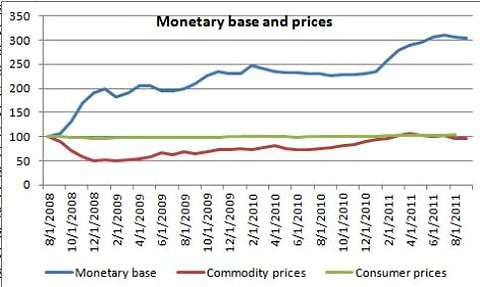
\includegraphics{img/100711krugman3-blog480.jpg}
    \caption{Entwicklung des Preises auf Basis der Geldmenge während der Finazkrise 08/09, \cite{Krugman2011}}
\end{figure}    

Eindeutig lässt sich dabei feststellen, dass obwohl die Geldmenge innerhalb der Krisenzeit, sowie auch danach, massiv auf das fast dreifache anstieg, es keine Veränderung bei den Preisen enstprechend der Inflationshypothese \vref{Inflationshyptothese} gab. Laut der Quantitätstheorie und der Geldnachfragefunktion \vref{Geldnachfragefunktion} müsste also auch der durchschnittliche Preis um einen äquivalenten Faktor ansteigen. In der Grafik ist allerdings zu erkennen, dass dieser Anstieg entgegen der Prognose der monetaristischen Inflationstheorie, nicht erfolgte.
